\documentclass[a4paper,10pt,titlepage]{article}

\usepackage{geometry}
\usepackage{amsmath}
\usepackage{amssymb}
\usepackage{txfonts}
\usepackage{microtype}
\usepackage{epsfig}
\usepackage{graphicx}
\usepackage{moreverb}
\usepackage{hyperref}
\usepackage{listings}
\usepackage{xcolor}
\usepackage{textcomp}
\definecolor{listinggray}{gray}{0.98}
\definecolor{lbcolor}{rgb}{0.98,0.98,0.98}
\lstset{
	backgroundcolor=\color{lbcolor},
	tabsize=4,
	rulecolor=,
	language=matlab,
    basicstyle=\scriptsize\ttfamily,
    upquote=true,
    aboveskip={1.5\baselineskip},
    columns=fixed,
    showstringspaces=false,
    extendedchars=true,
    breaklines=true,
    prebreak = \raisebox{0ex}[0ex][0ex]{\ensuremath{\hookleftarrow}},
    frame=single,
    showtabs=false,
    showspaces=false,
    showstringspaces=false,
    identifierstyle=\ttfamily,
    keywordstyle=\color[rgb]{0,0,1},
    commentstyle=\color[rgb]{0.133,0.545,0.133},
    stringstyle=\color[rgb]{0.627,0.126,0.941},
}
\usepackage{eso-pic}
\usepackage{ifthen}

\AddToShipoutPictureBG{\ifthenelse{\equal{\value{page}}{0}}{}{
\includegraphics{template_files/backgroundlines}}}


\usepackage{tikz}
\usepackage{pgfplots}
\usepackage{tikzscale}
\usepackage{graphicx}
\usepackage{float}
\usepackage{subcaption}
\usepackage{comment}
\usepackage{units}
\usetikzlibrary{external}\tikzexternalize


\title{H3b: Time dependent quantum mechanics}
\author{Victor Nilsson and Simon Nilsson (930128-1854)}
\date{\today}

\begin{document}

\newgeometry{top=2cm,bottom=2cm,left=2cm,right=2cm}

\begin{titlepage}

\setcounter{page}{0}

\begin{center}
{\huge \bf \color{red} NB: The graded, first version of the report must be
                           returned if you hand in a second time! } \\
\vspace{3cm}
\makeatletter
{ \huge \@title } \\
\vspace{1cm}
{ \Large \@author }\\
\vspace{1cm}
{ \Large \@date }\\
\makeatother
\end{center}

\vfill

\begin{flushright}
{\Large
\begin{tabular}{|c|c|c|}
\hline
Task N\textsuperscript{\underline{o}} & Points & Avail.\ points \\ \hline
\hspace{3cm} & \hspace{3cm} & \hspace{3cm} \\ \hline
~ & ~ & ~ \\ \hline
~ & ~ & ~ \\ \hline
~ & ~ & ~ \\ \hline
~ & ~ & ~ \\ \hline
~ & ~ & ~ \\ \hline
~ & ~ & ~ \\ \hline
~ & ~ & ~ \\ \hline
$\sum$ & ~ & ~ \\
\hline
\end{tabular}}
\end{flushright}

\end{titlepage}

\newgeometry{top=2cm,bottom=2cm,left=1.5cm,right=7.4cm}


\section*{Introduction}

\section*{Problem 1}

The initial distribution of the Gaussian wave packet,

\begin{equation}
	\psi(x;0)=\frac{1}{(\pi d^2)^{1/4}} \exp(-\frac{(x-x_0)^2}{2d^2}) \exp(i p_0(x-x_0)/\hbar),
\end{equation}

where $d$ is the witdth of the packet, $x_0$ and $p_0$ are the corresponding initial position and momenta.

\begin{figure}[H]
    \centering
    \captionsetup[subfigure]{justification=centering}
    \begin{subfigure}[b]{0.7\textwidth}
        \centering
        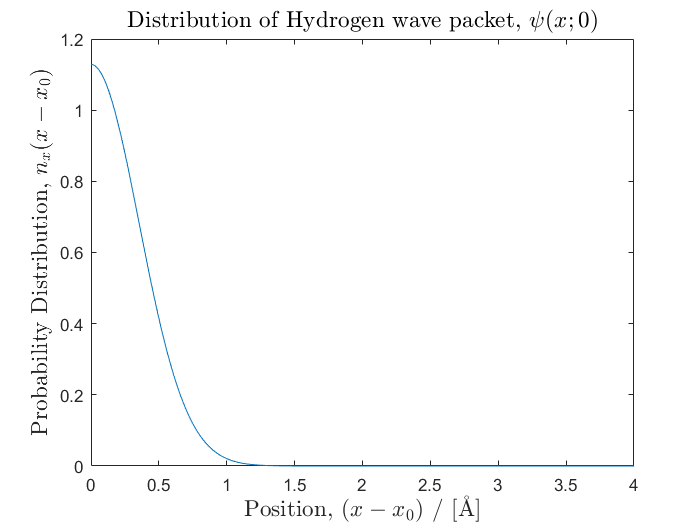
\includegraphics[width=\textwidth]{graphics/task1/position_prob.png}
		\caption{}
		\label{fig:*_a}
    \end{subfigure}
    \begin{subfigure}[b]{0.7\textwidth}
        \centering
        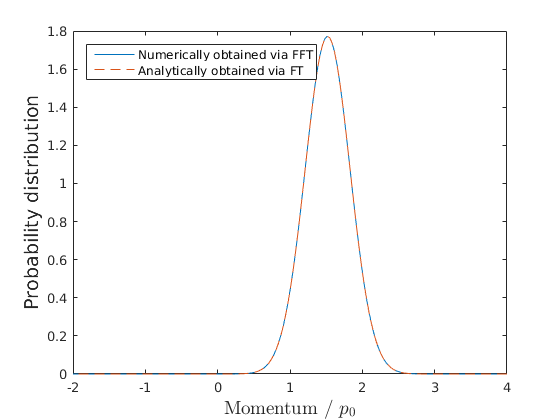
\includegraphics[width=\textwidth]{graphics/task1/momentum_prob.png}
        \caption{}
		\label{fig:*_b}
    \end{subfigure}
    \caption{\textit{(a):} * \textit{(b):} *}
    \label{fig:*}
\end{figure}

Fourier of the gaussian,

\begin{align}
	\mathcal{F}\left[\psi(x;0)\right](p) 							& =  \int_{-inf}^{inf} e^{-ipx} \psi(x;0) dx \\
 																	& = \frac{1}{(\pi d^2)^{1/4}}\int_{-inf}^{inf}e^{-ipx}e^{-\frac{(x-x_0)^2}{2d^2}} e^{ip_0(x-x_0)/\hbar}dx\\
\left\{a=\frac{e^{-ipx_0}}{(\pi d^2)^{1/4}}\right\}					& = a \int_{-inf}^{inf}e^{-ip(x-x_0)}e^{-\frac{(x-x_0)^2}{2d^2}}e^{ip_0(x-x_0)/\hbar} dx\\
\left\{
\begin{array}{ll}
x'	& = x-x_0\\
dx' & = dx   \\
x'	& \rightarrow x\\
\end{array}
\right\} 															& = a\int_{-inf}^{inf}e^{-i(p-p_0/\hbar)x}e^{-\frac{x^2}{2d^2}}dx \\
\left\{
\begin{array}{ll}
p'		& = p-p_0/\hbar\\
b		& = \frac{1}{2d^2}   \\
x'		& = x-\frac{ip}{2b}\\
dx'		& = dx\\
x'		& \rightarrow x\\
\end{array}
\right\}															& = a\int_{-inf}^{inf}e^{-bx^2}e^{-p'^2/4b} dx\\
																	& = ae^{-p'^2/4b}\int_{-inf}^{inf}e^{-bx^2} dx\\
\left\{\int_{-int}^{int}e^{-bx^2}dx=\sqrt{\frac{\pi}{2b}}\right\}	& = ae^{-p'^2/4b}\sqrt{\frac{\pi}{2b}}\\
																	& = (\pi d^2)^{1/4}e^{-ipx_0-(p\hbar-p_0)^2d^2/2\hbar^2}
\end{align}


\bibliography{references}
\bibliographystyle{plain}

\appendix
\section{Source code}

\subsection{\texttt{main1.m}}
\lstinputlisting[language=matlab, numbers=left]{../code/main1.m}

\subsection{\texttt{main2.m}}
\lstinputlisting[language=matlab, numbers=left]{../code/main2.m}

\subsection{\texttt{main3.m}}
\lstinputlisting[language=matlab, numbers=left]{../code/main3.m}

\subsection{\texttt{main4.m}}
\lstinputlisting[language=matlab, numbers=left]{../code/main4.m}

\end{document}
